\documentclass[11pt]{article}
\usepackage{amssymb}
\usepackage{amsthm}
\usepackage{amsmath}
\usepackage{listings}
\usepackage{color}
\usepackage{graphicx}
\usepackage[margin=1.0in]{geometry}

\lstdefinestyle{matlab-style}{
language=Matlab,
basicstyle=\scriptsize\ttfamily,
tabsize=2,
rulecolor=,
language=matlab,
basicstyle=\scriptsize,
aboveskip={1.5\baselineskip},
columns=fullflexible,
showstringspaces=false,
extendedchars=true,
breaklines=true,
prebreak = \raisebox{0ex}[0ex][0ex]{\ensuremath{\hookleftarrow}},
frame=single,
showtabs=false,
showspaces=false,
showstringspaces=false,
identifierstyle=\ttfamily,
keywordstyle=\color[rgb]{0,0,1},
commentstyle=\color[rgb]{0.133,0.545,0.133},
stringstyle=\color[rgb]{0.627,0.126,0.941},
keepspaces=true,
numbers=left,
numbersep=5pt,
numberstyle=\tiny\color[rgb]{0.5,0.5,0.5},
stepnumber=1
}

\title{Design of an optimal wing spar\\MANE 6963 - Project 2}
\author{ID: 2168}
\date{}

\begin{document}

\maketitle

\section{Executive summary}

In this report, we investigate the optimal design of a spar
as the primary support for the wing of an aircraft. Our
main objective is to minimize the weight of the wing spar
subject to specific design constraints, design assumptions,
and operational assumptions about the aircraft.

\begin{figure}[hbt]
\centering
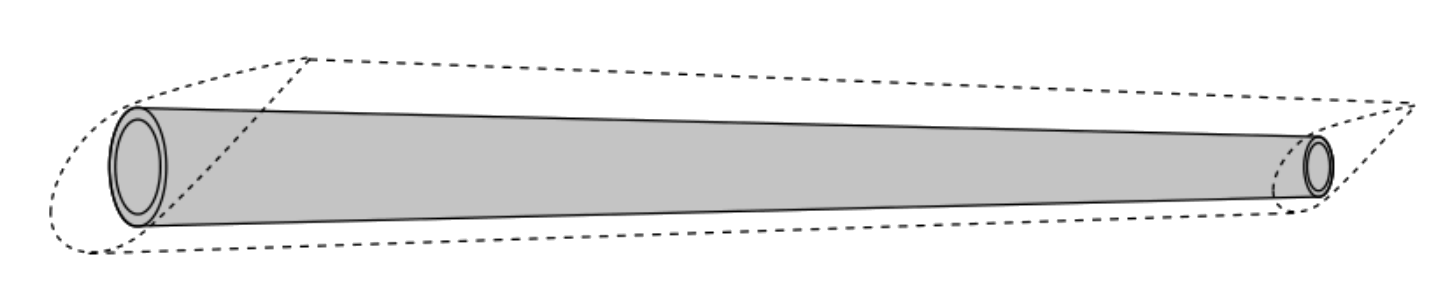
\includegraphics[width=0.6\textwidth]{spar}
\label{fig:spar}
\caption{Wing and illustration of spar geometry}
\end{figure}

\subsection{Aircraft operational assumptions}

\begin{figure}[hbt]
\centering
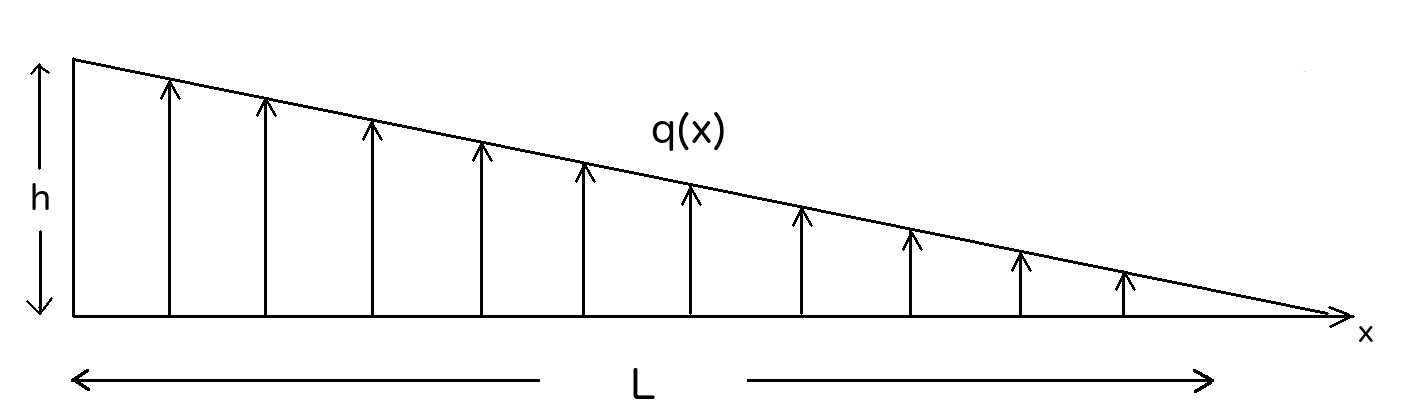
\includegraphics[width=0.6\textwidth]{load}
\caption{Load imposed on the wing}
\label{fig:load}
\end{figure}

We assume that the total mass of the aircraft is
$m_{\text{plane}} = 500$ kg and that the plane
is equally supported by two wings. 
Additionally, we assume that the wing semi-span,
which is also the length of the spar, is
$L = 7.5$ m. Finally,
we assume that the plane will be operating at
a $2.5$ g maneuver and that the span-wise force
distribution acting on the wing
(and thus on the spar) during this maneuver
is linearly varying, vanishing at the wing tip.
The distribution of the force per unit area $q(x)$
acting on the spar is shown in Figure \ref{fig:load}.

\subsection{Design assumptions}

We assume that the spar will be made of a composite
carbon fiber material with the material properties
shown in Figure \ref{fig:materials},
where the ultimate yield strength is equal in tension
and in compression.

\begin{figure}[hbt]
\centering
\begin{tabular}{ | l | r  |}
\hline
Material property & Value \\ \hline
Density $(\rho)$ & $1600$ km/m$^3$ \\ \hline
Young's modulus $(E)$ & $70$ GPa \\ \hline
Ultimate yield strength $(Y)$ & $600$ MPa \\ \hline
\end{tabular}
\caption{Material properties of the spar}
\label{fig:materials}
\end{figure}

The cross-sectional shape of the spar is assumed to a
circular annulus, as shown in Figure \ref{fig:section}.

\begin{figure}[hbt]
\centering
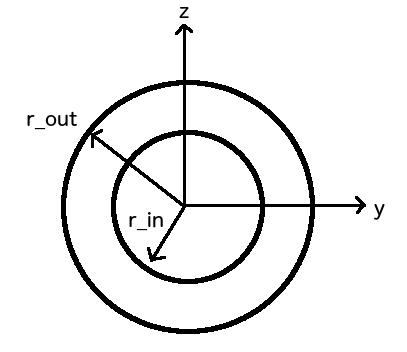
\includegraphics[width=0.3\textwidth]{annulus}
\caption{Cross-section of the spar geometry}
\label{fig:section}
\end{figure}

\subsection{Design constraints}

\section{Geometry representation}

\newpage

\section{Appendix: code listings}

\lstinputlisting[
  style=matlab-style,
  caption=CalcForce.m]{CalcForce.m}

\lstinputlisting[
  style=matlab-style,
  caption=CalcMomentInertia.m]{CalcMomentInertia.m}

\newpage

\lstinputlisting[
  style=matlab-style,
  caption=CalcWeight.m]{CalcWeight.m}

\end{document}
